%% LyX 2.3.2 created this file.  For more info, see http://www.lyx.org/.
%% Do not edit unless you really know what you are doing.
\documentclass[english]{colostatethesisLyx}
\usepackage[T1]{fontenc}
\usepackage[latin9]{inputenc}
\setcounter{secnumdepth}{3}
\setcounter{tocdepth}{3}
\usepackage{array}
\usepackage{units}
\usepackage{multirow}
\usepackage{amsbsy}
\usepackage{amstext}
\usepackage{graphicx}

\makeatletter

%%%%%%%%%%%%%%%%%%%%%%%%%%%%%% LyX specific LaTeX commands.
%% Because html converters don't know tabularnewline
\providecommand{\tabularnewline}{\\}

%%%%%%%%%%%%%%%%%%%%%%%%%%%%%% Textclass specific LaTeX commands.
\usepackage{amssymb}
\usepackage{graphicx}
\usepackage{url}

\makeatother

\usepackage{babel}
\begin{document}
This describes the thesis

\section{Introduction to Neutrinos}

The history of the neutrino can be traced back to electron energy
spectrum observed in neutron $\beta$-decay. While measurements of
$\alpha$- and $\gamma$-decay of atomic nuclei showed discrete spectral
lines, the electron ($\beta$ particle) exhibited a continuous energy
spectrum. Experimentally, there were two observed particles in each
decay process and classical physics dictated that the outgoing daughter
particles should have discrete energies. The fact that the $\beta$-decay
spectrum was not this way posed a fundamental problem for physicists
in the mid-1910s and later, was energy conserved? Two solutions were
postulated: either the ``energy conservation law is only valid statistically
in such a process {[}...{]} or an additional undetectable new particle
{[}...{]} carrying away the additional energy and spin {[}...{]} is
emitted \cite{Zuber2012}.'' The latter solution was supported by
Wolfgang Pauli in a letter dated 4 December 1930 to a group of physicists
meeting in T�bingen, modern Germany, where he first proposed what
we would call a neutrino today\footnote{In W Pauli's December 1930 letter, he referred to his proposed particle
as the ``neutron'', which is not the same neutron we know of today.
At that point in time, the neutral particles inside the atomic nucleus,
also called ``neutrons'', had not been discovered, let alone understood.
The neutron, which was discovered in 1932 by James Chadwick, has been
formally associated as the neutral, cousin particle to the proton.
It would be Enrico Fermi who would coin the particle in W Pauli's
letter and solution to the $\beta$-decay spectrum a ``neutrino'',
meaning \textit{little neutral one}.}. Pauli's solution also predicted that the undetected neutrino would
have half-integer spin, a quantum mechanical property of matter, since
the observed particles in $\beta$-decay did not conserve angular
momentum. The existence of the neutrino and validation of Pauli's
predictions would not experimentally verified for another 20 years. 

The neutrino was first discovered in 1953 by Clyde Cowan and Frederick
Reines using a nuclear reactor in South Carolina, U.S.A.. Since then
three types of neutrinos have been observed and from unique sources
like the Sun and a supernova. Neutrino physics continues to be an
active region of physics since neutrinos are unique probes to processes
otherwise inaccessible in laboratories. For instance in the depths
of the Sun's core where fusion occurs and neutrinos are created, neutrinos
are able to travel through the ultra dense and hot medium of the core
(over $10^{7}$ degrees Kelvin) and outer layers of the Sun and reach
us on Earth. 

Neutrinos rarely interact with normal matter, meaning that they travel
essentially unimpeded towards one's particle detector. The rarity
of such interactions can be illustrated with the fact that given nearly
$7.0\times10^{10}\text{ neutrinos}/\text{cm}^{2}/\text{sec}$\footnote{To give some perspective to this number, this means 70 billion neutrinos
are travelling every second through an area similar to one's own thumb
nail.} are incident on the Earth from the Sun, statistically one solar neutrino
can harmlessly interact with an individual. So this begs the question:
how does one detect a neutrino? The short answer is one needs a ultra
large volume of matter and a large enough flux of neutrinos in its
path just to detect one given today's technology. 

Scientists continue to be interested in neutrinos due to properties
they exhibit. One of the more recent and surprising aspects about
neutrinos is their ability to undergo ``flavor oscillations'' where
a neutrino of definite flavor (type) is created and later observed
as a different flavor. The impact of such oscillations could help
explain the observed matter and anti-matter asymmetry in the Universe. 

\subsection{Neutrinos in the Standard Model}

The Standard Model (SM) of particle physics is the theory that describes
the electromagnetic, strong nuclear, and weak nuclear forces and the
elementary particles therein. These three forces and the gravitational
force constitute the four \textit{known} fundamental forces of the
Universe. Each force in the SM has at least one ``force carrier''
particle that mediates the interactions between particles. The force
carriers are formally called gauge bosons which indicates they are
particles with integer $(0,1,2,...)$ spin. The weak nuclear gauge
bosons, the W and Z, couple to neutrinos as well as the other fermions,
particles with half-integer $\left(\frac{1}{2},\frac{3}{2},\frac{5}{2},...\right)$
spin, in the SM. All the elementary particles of the SM are shown
in Figure \ref{fig:TheStandardModel}.

\begin{figure}
\begin{centering}
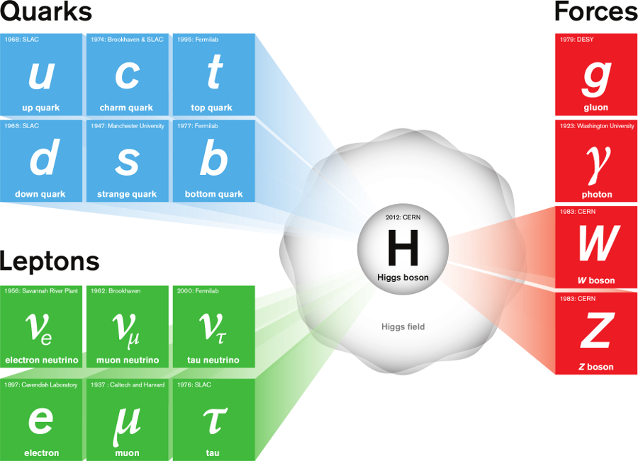
\includegraphics[height=0.17\textheight]{Figures/Introduction/StandardModel}
\par\end{centering}
\caption[The Standard Model of particle physics]{The Standard Model of particle physics consists of six quarks (up,
down, strange, charm, bottom, and top), six leptons (electron, muon,
tau, electron neutrino, muon neutrino, and tau neutrino), four force
propagating bosons (gluon, photon, W, and Z), and the Higgs boson.
The quarks, electron, muon, tau, W, and Z all gain mass through the
Higgs field. The focus of this thesis are the neutrinos which are
classified according to their charged, more massive Lepton cousins.
Image taken from \cite{Adams:2013qkq}. \label{fig:TheStandardModel}}
\end{figure}

Neutrinos in the SM are electrically neutral, massless particles categorized
into three generations based on their charged, more massive Lepton
cousins. They are believed to follow the free-particle Dirac Equation
which is given by
\begin{equation}
\left[i\hbar\sum_{\mu=0}^{3}\gamma^{\mu}\partial_{\mu}-mc\right]\psi=0\label{eq:diraceqn}
\end{equation}
where
\begin{equation}
\gamma^{0}=\begin{bmatrix}I_{2} & 0\\
0 & -I_{2}
\end{bmatrix},\gamma^{1}=\begin{bmatrix}0 & \sigma_{x}\\
-\sigma_{x} & 0
\end{bmatrix},\gamma^{2}=\begin{bmatrix}0 & \sigma_{y}\\
-\sigma_{y} & 0
\end{bmatrix},\gamma^{3}=\begin{bmatrix}0 & \sigma_{z}\\
-\sigma_{z} & 0
\end{bmatrix},\label{eq:gammamatrices}
\end{equation}
$I_{2}$ is the $2\times2$ identity matrix, $\sigma_{x,y,z}$ are
the Pauli Spin matrices, and
\begin{equation}
\partial_{0}=\frac{1}{c}\partderiv t,\partial_{1}=\partderiv x,\partial_{2}=\partderiv y,\partial_{3}=\partderiv z.\label{eq:fourderivative}
\end{equation}
The solutions to \eqref{eq:diraceqn} are called Dirac spinors and
can be written in terms of left-handed (LH) and right-handed (RH)
components. Any spinor can be decomposed in LH and RH projections
using a ``chiral'' operator $\hat{O}$ as
\begin{equation}
\psi=\left(\hat{O}_{\text{LH}}+\hat{O}_{\text{RH}}\right)\psi.\label{eq:chiralprojections}
\end{equation}
The chiral operators $\hat{O}_{\text{LH,RH}}$ in \eqref{eq:chiralprojections}
are defined as
\begin{equation}
\hat{O}_{\text{LH}}\psi=\frac{1}{2}(I_{4}-\gamma^{5})\psi=\psi_{\text{LH}}\quad\hat{O}_{\text{RH}}\psi=\frac{1}{2}(I_{4}+\gamma^{5})\psi=\psi_{\text{RH}}\label{eq:chiraloperators}
\end{equation}
where $I_{4}$ is the $4\times4$ identity matrix,
\begin{equation}
\gamma^{5}=i\gamma^{0}\gamma^{1}\gamma^{2}\gamma^{3}=\begin{bmatrix}0 & I_{2}\\
I_{2} & 0
\end{bmatrix},\label{eq:gammafivedef}
\end{equation}
and $\psi_{\text{LH,RH}}$ are LH and RH chiral spinors. Using \eqref{eq:chiraloperators},
the Dirac Equation then becomes after some manipulation
\begin{equation}
\begin{aligned}i\hbar\left(\frac{1}{c}\partderiv t-\boldsymbol{\sigma}\cdot\boldsymbol{\nabla}\right)\psi_{\text{RH}} & =m\gamma^{0}\psi_{\text{LH}}\\
i\hbar\left(\frac{1}{c}\partderiv t+\boldsymbol{\sigma}\cdot\boldsymbol{\nabla}\right)\psi_{\text{LH}} & =m\gamma^{0}\psi_{\text{RH,}}
\end{aligned}
\label{eq:diraceqnchiral}
\end{equation}
where
\begin{equation}
\boldsymbol{\sigma}\cdot\boldsymbol{\nabla}=\sum_{i=1}^{3}\sigma_{i}\nabla_{i}.\label{eq:matrixdotproduct}
\end{equation}
In the limiting case of vanishing mass $\left(m\rightarrow0\right)$,
as in the SM, the free particle equations decouple into
\begin{equation}
\begin{aligned}\left(\frac{E}{c}-\boldsymbol{\sigma}\cdot\boldsymbol{P}\right)\psi_{\text{RH}} & =0\\
\left(\frac{E}{c}+\boldsymbol{\sigma}\cdot\boldsymbol{P}\right)\psi_{\text{LH}} & =0.
\end{aligned}
\quad\left[\text{Momentum basis}\right]\label{eq:diraceqnchiralmassless}
\end{equation}
We now have enough information to make two very important insights
about neutrinos in the SM.

The first important insight is that the chirality and helicity of
the neutrino the same for $m\rightarrow0$. A particle's helicity
is the projection of the spin vector on its momentum vector given
as
\begin{equation}
\mathcal{H}=\frac{\boldsymbol{\sigma}\cdot\mathbf{P}}{\left|\mathbf{P}\right|}\label{eq:helicityoperator}
\end{equation}
where $\boldsymbol{\sigma}$ is the spin vector and $\mathbf{P}$
is the 3-momentum of the particle. Since \eqref{eq:diraceqnchiralmassless}
commutes $\left(\left[\hat{A},\hat{B}\right]=\hat{A}\hat{B}-\hat{B}\hat{A}\right)$
with $\mathcal{H},$ $\psi_{\text{LH,RH}}$ are eigenstates of the
helicity operator with eigenvalues $\pm1$.

The second important fact is that a weakly interacting neutrino has
positive energy $E=\left|\boldsymbol{P}\right|c$ and is always LH
as shown in \eqref{eq:chiraloperators}. The antineutrino is RH and
has negative energy $(-E=\left|\boldsymbol{P}\right|c)$ which is
interpreted to mean it travels backwards in time. Since neutrinos
are nearly massless, there are no mechanisms for RH neutrinos and
LH antineutrinos. The helicity of the neutrino is visualized in Figure
\ref{fig:DecayOfPion} which shows the decay of a pion at rest into
a muon and neutrino. Since a pion has net zero (0) spin, the spin
vectors of the daughters must also sum to zero. The neutrino's helicity
(-1) and hence LH chirality is inferred by the positively charged
muon of which has +1 helicity. To confirm the antineutrino's RH chirality
(+1) requires both a charge (C) conjugation and parity (P) transformation.
A C conjugation transforms all particles into their corresponding
antiparticles while P transformation inverts all spatial coordinates.
\begin{figure}
\begin{centering}
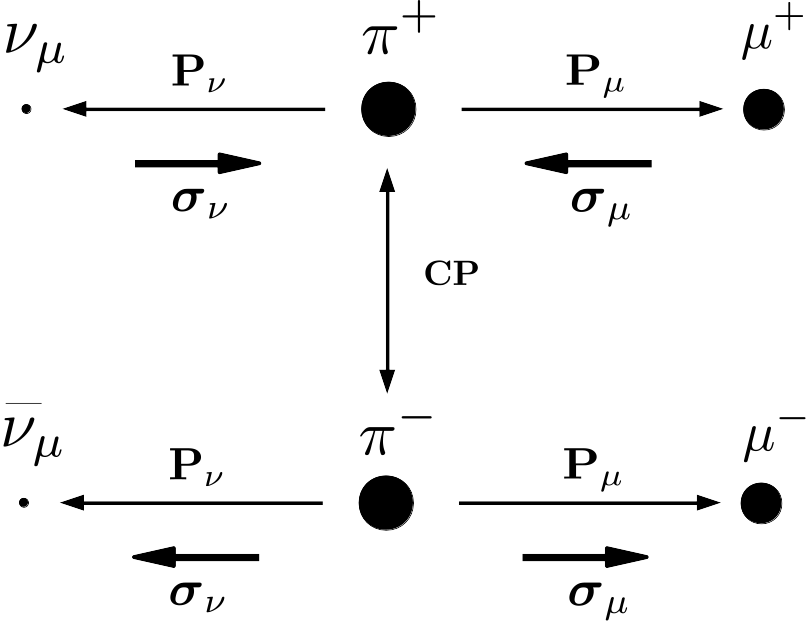
\includegraphics[width=0.5\textwidth]{Figures/Introduction/ChiralityPionDecay}
\par\end{centering}
\caption[Helicity of Neutrino Through Decay of Charged Pi Mesons]{Decay of a charged pi meson into a muon and neutrino show the direction
of the momentum $\boldsymbol{P}$ and spin $\boldsymbol{\sigma}$
of the outgoing particles. Since a pion at rest has zero (0) angular
momentum, the system of daughter particles must have net zero angular
momentum as well. A neutrino (antineutrino) is a right- (left-) handed
helicity particle since its spin is (anti-)parallel to its momentum.
Application of charge and parity (CP) converts all the particles into
their respective antiparticles.\label{fig:DecayOfPion}}

\end{figure}
 

The observation of only LH neutrinos and RH antineutrinos are an important
feature in the SM. The weak force allows for P and CP violation due
to its vector minus axial-vector (V-A) construction which is how a
LH neutrino is described in \eqref{eq:chiraloperators}. Further observation
of CP violation is being explored with neutrinos through a process
called neutrino oscillations. This will be explained in the next subsection.

\subsection{Neutrino Oscillations}

Neutrino oscillations are the observation of a neutrino produced of
definite flavor and later observed as a different flavor. A deficit
of neutrinos were observed for a number of atmospheric and solar neutrino
experiments and the effect became more pronounced as the distance
from the source increased.

The first indication of neutrino oscillations was from the Ray Davis
Homesteak Mine experiment which began in the 1960s. Ray Davis was
an expert Chemist and designed a radiochemical experiment to measure
the flux of neutrinos from Sun. The purpose of this experiment was
to test John Bahcall's prediction of the fusion rate in and neutrino
flux from the Sun. Measurements continued into the 1980s and showed
that the flux of neutrinos as measured at Homesteak was about 1/3
the expected rate and became known as the ``Solar Neutrino Problem.''
The primary solutions were either the neutrino capture cross section
is lacking or the solar model was incorrect. The Sudbury Neutrino
Observatory (SNO) was able to resolve this by making a model-independent
measurement of the solar neutrino flux. The SNO $\nue$CC/NC ratio
is given by $0.301\pm0.033$, which confirmed that only 30\% of neutrinos
arrive as $\nue$ on Earth, firmly established that the majority of
neutrinos arrive as the wrong flavor.

Another outstanding problem emerged with measurements of atmospheric
neutrinos, in particular muon and electron types. Atmospheric neutrinos
are produced when high energy cosmic rays strike atmospheric particles.
These cosmic ray collisions generate mostly pions and kaons that decay
into neutrinos. When trying to measure the $\numu/\nue$ ratio and
comparing that with expected ratio, there was a significant deficit.
This was particularly a problem as a function of the zenith angle
for the Super-Kamiokande experiment.

While the phenomenon of neutrino oscillations has understood for decades,
it is not incorporated into the SM since oscillations require the
neutrino has mass. The reasons why neutrino oscillations require massive
neutrinos is explained in the next subsection.

\subsubsection{Two Flavor Derivation}

The phenomenon of neutrino oscillations can be described with elementary
Quantum Mechanics. Beginning with the Schr�dinger Equation in \eqref{eq:schroeqn}

\begin{equation}
\begin{aligned}-\frac{\hbar}{i}\partderiv t\diracket{\nu(\mathbf{r},t)} & =\hat{H}\diracket{\nu(\mathbf{r},t)}\end{aligned}
\label{eq:schroeqn}
\end{equation}
where $\hat{H}$ is the Hamiltonian for the physical system. If we
consider a massive neutrino of mass $m_{j}$ in its rest frame (free
particle), the Hamiltonian becomes diagonal which acting on $\diracket{\nu_{j}}$
results in the eigenvalue equation

\begin{equation}
\hat{H}\diracket{\nu_{j}(\mathbf{r},t)}=E_{j}\diracket{\nu_{j}(\mathbf{r},t)}\label{eq:schroeqntimeindep}
\end{equation}
where $E_{j}$ is the energy of the neutrino $\diracket{\nu_{j}}$.
If we substitute \eqref{eq:schroeqntimeindep} into \eqref{eq:schroeqn}
and solve for $\diracket{\nu(\mathbf{r},t)}$, we obtain the following

\begin{equation}
\diracket{\nu_{j}(\mathbf{r},t)}=e^{-iE_{j}t/\hbar}\diracket{\nu_{j}(\mathbf{r},t=0)}\label{eq:schroeqnsolution}
\end{equation}
where $\diracket{\nu_{j}(\mathbf{r},t=0)}$ is created with momentum
$\mathbf{p}$ at the origin $\mathbf{r}=0$. The time-independent
solution to \eqref{eq:schroeqn} is a plane-wave given by
\begin{equation}
\diracket{\nu_{j}(\mathbf{r},t=0)}=e^{i\mathbf{p}\cdot\mathbf{r}/\hbar}\diracket{\nu_{j}}.\label{eq:schroeqnsolutiontimeindep}
\end{equation}
Before being able to describe neutrino oscillations, we must define
our basis states. For this example, consider that there are only two
eigenstates, labeled $\nu_{1}$ and $\nu_{2}$, in the ``mass''
basis with definite mass $m_{1}$ and $m_{2}$, respectively. However,
experiments can produce neutrinos, as well as probe them, only of
definite ``flavor'', denoted by a Greek letter subscript $\lambda$.
Let the generated neutrino, which is a linear superposition of mass
states 1 and 2, have momentum $\mathbf{p}$ and flavor $\alpha$.
Since both mass eigenstates share the same momentum momentum $\mathbf{p}$
(but not energy!), the exponential term in \eqref{eq:schroeqnsolutiontimeindep}
is an overall phase that will cancel out later. We can postulate a
linear transformation, $U$, between the basis states given by \eqref{eq:pmnstwodimgen}.

\begin{equation}
\begin{bmatrix}\nu_{\alpha}\\
\nu_{\beta}
\end{bmatrix}=\begin{bmatrix}U_{11} & U_{12}\\
U_{21} & U_{22}
\end{bmatrix}\begin{bmatrix}\nu_{1}\\
\nu_{2}
\end{bmatrix}\label{eq:pmnstwodimgen}
\end{equation}
This linear transformation must be a unitary matrix $\left(U^{-1}=U^{\dagger},\dagger=\text{transpose conjugate}\right)$
since the states $\nu_{1,2}$ constitute a complete orthonormal set
in the mass basis. With this unitary property, we can imagine $U$
as a rotation matrix

\begin{equation}
\begin{bmatrix}\nu_{\alpha}\\
\nu_{\beta}
\end{bmatrix}=\begin{bmatrix}\begin{array}{rr}
\cos(\theta) & \sin(\theta)\\
-\sin(\theta) & \cos(\theta)
\end{array}\end{bmatrix}\begin{bmatrix}\nu_{1}\\
\nu_{2}
\end{bmatrix},\label{eq:pmnstwodimangle}
\end{equation}
where $\theta$ is the angle between the two bases. We can imagine
this transformation between bases as shown in Figure \ref{fig:twoflavorrotation}.
If we create a neutrino of flavor $\alpha$ and observe it after a
time $t=T>0$, then the probability of observing it as flavor $\beta\neq\alpha$
is given by
\begin{flushleft}
\begin{figure}
\begin{centering}
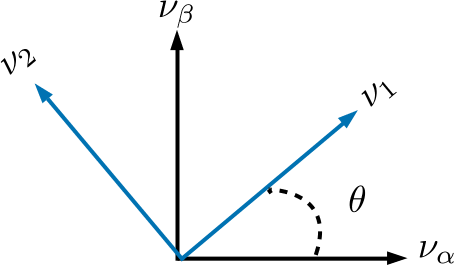
\includegraphics[scale=0.5]{Figures/Introduction/RotationMatrix}
\par\end{centering}
\caption[Depiction of Two Neutrino Flavor Change of Basis]{The depiction of two neutrino flavor change of basis using a rotation
matrix. Compare this with \eqref{eq:pmnstwodimangle}.\label{fig:twoflavorrotation}}

\end{figure}
\begin{equation}
\begin{aligned}\mathcal{P}\left(\nu_{\alpha}\rightarrow\nu_{\beta}\right) & =\left|\braket{\nu_{\alpha}(t=0)|\nu_{\beta}(t=T)}\right|^{2}\\
 & =\left|\left(\cos(\theta)\diracbra{\nu_{1}(t=0)}+\sin(\theta)\diracbra{\nu_{2}(t=0)}\right)\right.\\
 & \ \ \ \ \times\left.\left(-\sin(\theta)\diracket{\nu_{1}(t=T)}+\cos(\theta)\diracket{\nu_{2}(t=T)}\right)\right|^{2}\\
 & =\left|\braket{\nu_{1}(0)|\nu_{1}(T)}(-cs)+\braket{\nu_{1}(0)|\nu_{2}(T)}(cc)\right.\\
 & \ \ \ \ \left.+\braket{\nu_{2}(0)|\nu_{1}(T)}(-ss)+\braket{\nu_{2}(0)|\nu_{2}(T)}(sc)\right|^{2}
\end{aligned}
\label{eq:prob2flavorexpanded}
\end{equation}
where for simplicity $c=\cos(\theta)$ and $s=\sin(\theta)$. Evaluating
all inner products and simplifying terms in \eqref{eq:prob2flavorexpanded}
results in \eqref{eq:prob2flavorsimplified} below.
\par\end{flushleft}

\begin{equation}
\mathcal{P}\left(\nu_{\alpha}\rightarrow\nu_{\beta}\right)=\sin^{2}(2\theta)\sin^{2}\left(\frac{E_{1}-E_{2}}{2\hbar}T\right)\label{eq:prob2flavorsimplified}
\end{equation}

The terminology of ``neutrino oscillations'' should be more apparent
now since \eqref{eq:prob2flavorsimplified} demonstrates that the
probability changes sinusoidally. This equation is not, however, terribly
useful in the laboratory frame since it is hard to make an experiment
where the travel time an individual neutrino is well known. Instead,
we can make useful approximations that are accessible in the laboratory
frame. Since neutrinos are nearly massless, they travel very close
to the speed of light. Therefore we can replace time $T$ with $L/c$
where $L$ is the distance between the neutrino origin and detection
and $c$ is now the speed of light in vacuum. We can also approximate
the energy of the mass eigenstate as 

\begin{equation}
\begin{aligned}E_{j} & =\left(m_{j}^{2}c^{4}+p_{j}^{2}c^{2}\right)^{\frac{1}{2}}=p_{j}c\left(1+\frac{m_{j}^{2}c^{2}}{p_{j}^{2}}\right)^{\frac{1}{2}}\\
 & \approx p_{j}c\left(1+\frac{m_{j}^{2}c^{2}}{2p_{j}^{2}}+\mathcal{O}\left(\frac{m_{j}c}{p_{j}}\right)^{4}\right)\\
 & \approx E_{\nu}+\frac{m_{j}^{2}c^{4}}{2E_{\nu}},
\end{aligned}
\label{eq:enuapprox}
\end{equation}
where we have used the fact that $p_{j}\gg m_{j}c$ and $p_{j}c\approx E_{\nu}$
where $E_{\nu}$ is the neutrino energy as measured in the laboratory.
Substituting all of our assumptions in \eqref{eq:prob2flavorsimplified},
we get \eqref{eq:prob2flavorapprox}

\begin{equation}
\begin{aligned}\mathcal{\mathcal{P}}\left(\nu_{\alpha}\rightarrow\nu_{\beta}\right) & =\sin^{2}(2\theta)\sin^{2}\left(\frac{\Delta m^{2}c^{3}}{4\hbar}\frac{L}{E_{\nu}}\right),\end{aligned}
\label{eq:prob2flavorapprox}
\end{equation}
where $\Delta m^{2}=m_{2}^{2}-m_{1}^{2}$ is the mass-squared difference
between the mass states. If we evaluate all the physical constants
in natural units ($c=\hbar=1)$ and choose appropriate units for $\Delta m^{2}$,
$L$, and $E_{\nu}$, we arrive at the following expression

\begin{equation}
\mathcal{\mathcal{P}}\left(\nu_{\alpha}\rightarrow\nu_{\beta}\right)=\sin^{2}(2\theta)\sin^{2}\left(1.27\frac{\Delta m^{2}}{\left[\text{eV}^{2}\right]}\frac{\nicefrac{L}{E_{\nu}}}{\left[\nicefrac{\text{km}}{\text{GeV}}\right]}\right)\text{ [natural units]}\label{eq:prob2flavorapproxnaturalunits}
\end{equation}
which more clearly demonstrates the Physics in oscillations. The oscillation
probability has an amplitude of $\sin^{2}(2\theta)$ and varies with
frequency inversely proportional to $\Delta m^{2}$ as illustrated
in Figure \ref{fig:Two-flavor-oscillation}. Since $L$ and $E_{\nu}$
are the only controllable parameters for an oscillation experiment,
probing $\theta$ or $\Delta m^{2}$ can be difficult unless the experiment
can probe a large range of $L/E_{\nu}$ as shown in Figure \ref{fig:Two-flavor-oscillation-2}.

\begin{figure}
\begin{centering}
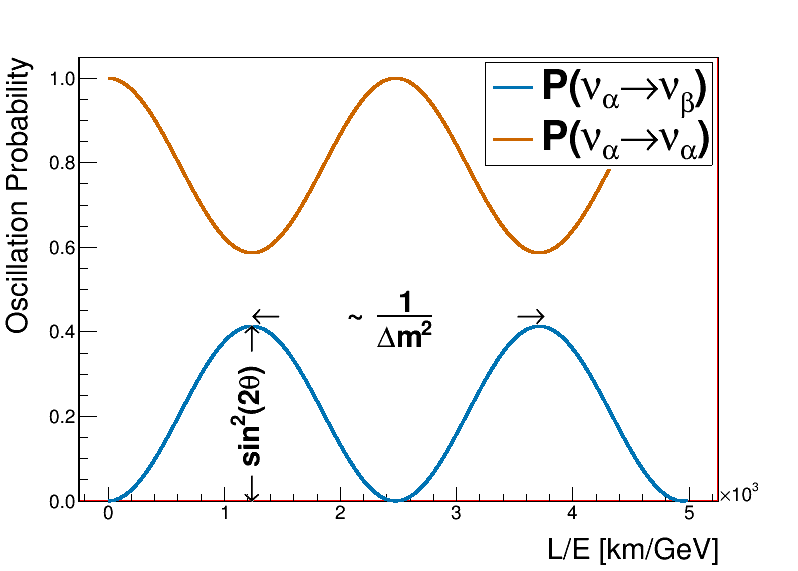
\includegraphics[width=0.49\textwidth]{Figures/Introduction/TwoNeutrinoOscillations}
\par\end{centering}
\caption[Survival and Disappearance Probability]{Two flavor oscillation probability as a function $L/E$ is shown
using $\theta=20^{\circ}$ and $\Delta m^{2}=\unit[10^{-3}]{eV^{2}}$.
The spacing between adjacent peaks/troughs is proportional to the
inverse of $\Delta m^{2}$. Note that $\mathcal{P}\left(\nu_{\alpha}\rightarrow\nu_{\alpha}\right)=1-\mathcal{P}\left(\nu_{\alpha}\rightarrow\nu_{\beta}\right)$
since the oscillation probability must always sum to 1.\label{fig:Two-flavor-oscillation}}
\end{figure}

\begin{center}
\begin{figure}
\begin{centering}
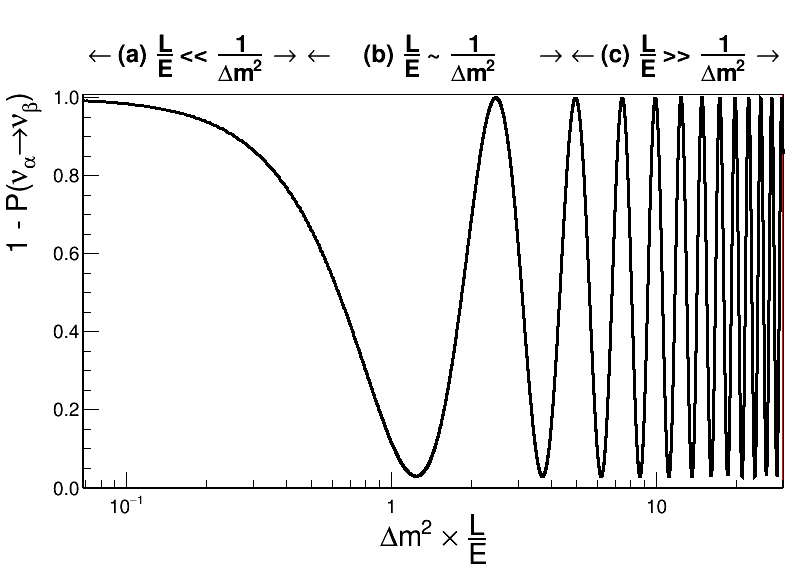
\includegraphics[width=0.49\textwidth]{Figures/Introduction/OscillationProb2FlavorLog}
\par\end{centering}
\caption[Logarithmic Plot of the Two Flavor Survival Probability]{Logarithmic plot of the survival probability $\left(1-\mathcal{P}\left(\nu_{\alpha}\rightarrow\nu_{\beta}\right)=\mathcal{P}\left(\nu_{\alpha}\rightarrow\nu_{\alpha}\right)\right)$
over a wide range of $L/E$ values for $\theta=40^{\circ}$. The arrows
above the plot roughly denote three possible cases: (a) no oscillations
($L/E\ll1/\Delta m^{2})$; (b) sensitivity to oscillations $(L/E\sim1/\Delta m^{2})$;
(c) only average measurement $(L/E\gg1/\Delta m^{2})$. Image originally
inspired by \cite{Schmitz1997}.\label{fig:Two-flavor-oscillation-2}}
\end{figure}
\par\end{center}

\subsubsection{Three Flavor Oscillations}

In the general case of oscillations using a $n\times n$ mixing matrix,
the unitary transformation can be written as a rotation matrix with
$\frac{n}{2}(n-1)$ weak mixing angles with $\frac{1}{2}(n-2)(n-1)$
Charge-Parity (CP) violating phases. In addition, oscillations are
dictated by a total of $n-1$ mass-squared splittings\cite{Zuber2012}.
This all assumes that neutrinos obey the Dirac Equation, or that they
are not their own antiparticles. The flavored mixing model is the
$3\times3$ matrix since there are three known neutrino flavors, $\nue$,
$\numu$, and $\nutau$, which means there are three (3) mixing angles,
one (1) CP violating phase, and two (2) mass-squared splittings. 

The most frequently used matrix parameterization is the Maki-Nakagawa-Sakata-Pontecorvo
(MNSP) matrix. Pontecorvo is accredited for first conceiving of neutrino
oscillations, albeit between neutrino and anti-neutrinos\cite{Ponte1957}.
It was Maki, Nakagawa, and Sakata who conceived of the parameterization
based off the ideas of Pontecorvo\cite{Maki1962}. The MNSP matrix
is decomposed into separate rotation matrices as given by \ref{eq:mnspdecomposed}
\begin{equation}
\begin{aligned}U_{\text{MNSP}} & =\stackrel{U_{\text{atm}}}{\overbrace{\begin{bmatrix}\begin{array}{rrr}
1 & 0 & 0\\
0 & c_{32} & s_{32}\\
0 & -s_{32} & c_{32}
\end{array}\end{bmatrix}}}\times\stackrel{U_{\text{rea}}}{\overbrace{\begin{bmatrix}c_{31} & 0 & s_{31}e^{i\delta_{\text{CP}}}\\
0 & 1 & 0\\
-s_{31}e^{-i\delta_{\text{CP}}} & 0 & c_{31}
\end{bmatrix}}}\times\stackrel{U_{\text{sol}}}{\overbrace{\begin{bmatrix}\begin{array}{rrr}
c_{21} & s_{21} & 0\\
-s_{21} & c_{21} & 0\\
0 & 0 & 1
\end{array}\end{bmatrix}}}\end{aligned}
\label{eq:mnspdecomposed}
\end{equation}
where 
\begin{equation}
\cc{ij}=\cos\theta_{ij},\ss{ij}=\sin\theta_{ij},\label{eq:cossinshorthand}
\end{equation}
and $\delta_{\text{CP}}$ represents the CP violating phase. Each
rotation matrix represents the different sources for neutrino oscillations
experiments with ``atm'', ``rea'', and ``sol'' representing
atmospheric $\nu$'s, nuclear reactor $\nu$'s, and Solar $\nu$'s,
respectively. The sensitivity of neutrino oscillations for different
sources is given in Table \ref{tab:SensitivityOscill}.
\begin{table}
\begin{centering}
\begin{tabular}{lclcl}
\hline 
Source & Species & $\overline{E}$ {[}GeV{]} & $L$ {[}km{]} & $\min\left(\Delta m^{2}\right)\ \left[\text{eV}^{2}\right]$ \tabularnewline
\hline 
\hline 
Reactor & $\antinue$ & $\sim10^{-3}$ & $1$ & $\sim10^{-3}$\tabularnewline
Reactor & $\antinue$ & $\sim10^{-3}$ & $100$ & $\sim10^{-5}$\tabularnewline
Accelerator & $\numu,\antinumu$ & $\sim1$ & $1$ & $\sim1$\tabularnewline
Accelerator & $\numu,\antinumu$ & $\sim1$ & $10^{3}$ & $\sim10^{-3}$\tabularnewline
Atmospheric $\nu$'s & $\nuparticle{e,\mu},\antinuparticle{\mu,e}$ & $\sim1$ & $10^{4}$ & $\sim10^{-4}$\tabularnewline
Sun & $\nue$ & $\sim10^{-3}$ & $1.5\times10^{8}$ & $\sim10^{-11}$\tabularnewline
\hline 
\end{tabular}
\par\end{centering}
\caption[Sensitivity of Different Oscillation Experiments]{Sensitivity of different oscillation experiments originally published
in\cite{Tanabashi2018}.\label{tab:SensitivityOscill}}
\end{table}

If neutrinos are their own antiparticles, they do not follow the Dirac
Equation but do follow the Majorana Equation. This adds two (in general
$n-1$) more CP violating phases to the MNSP matrix

\begin{equation}
U_{\text{MNSP}}\rightarrow\eqref{eq:mnspdecomposed}\times\stackrel{U_{\text{Majorana}}}{\overbrace{\begin{bmatrix}1 & 0 & 0\\
0 & e^{i\alpha} & 0\\
0 & 0 & e^{i\beta}
\end{bmatrix}}}\label{eq:mnspdecomposedmajorana}
\end{equation}
Unfortunately, neutrino oscillations are not able to probe the Majorana
phases since the Majorana matrix is diagonal. The question of if neutrinos
are Majorana ($\nu=\overline{\nu})$ or Dirac ($\nu\neq\overline{\nu})$
particles is an open question and is being explored by non-oscillation
experiments. The full three flavor oscillation probability is given
by
\begin{equation}
\begin{aligned}\mathcal{P}\left(\nu_{\alpha}\rightarrow\nu_{\beta}\right)=\delta_{\alpha\beta}-4 & \sum_{j=1}^{3}\left[\sum_{i>j}^{3}\text{Re}\left(K_{\alpha\beta,ij}\right)\sin^{2}\left(\phi_{ij}\right)\right]\\
+4 & \sum_{j=1}^{3}\left[\sum_{i>j}^{3}\text{Im}\left(K_{\alpha\beta,ij}\right)\sin\left(\phi_{ij}\right)\cos\left(\phi_{ij}\right)\right]
\end{aligned}
\label{eq:threeflavorprobgeneral}
\end{equation}
where
\begin{equation}
K_{\alpha\beta,ij}=U_{\alpha i}U_{\beta_{i}}^{*}U_{\alpha j}^{*}U_{\beta j}\label{eq:threeflavorprobgeneralK}
\end{equation}
and
\begin{equation}
\phi_{ij}=\frac{\Dm ijc^{3}}{4\hbar}\frac{L}{E_{\nu}}.\label{eq:threeflavorprobgeneralphi}
\end{equation}
As an example, consider the survival probability of a muon type neutrinos
is given by 
\begin{equation}
\begin{aligned}\mathcal{P}\left(\numu\rightarrow\numu\right)=1-4 & \sss{23}\ccc{13}\left(V_{\cos\delta_{\text{CP}}}\right)\sin^{2}\phi_{31}\\
-4 & \sss{23}\ccc{13}\left(W_{\cos\delta_{\text{CP}}}\right)\sin^{2}\phi_{32}\\
-4 & \left(V_{\cos\delta_{\text{CP}}}\right)\left(W_{\cos\delta_{\text{CP}}}\right)\sin^{2}\phi_{21}
\end{aligned}
\label{eq:numu2numuthreeflavorfull}
\end{equation}
where
\begin{equation}
V_{\cos\delta_{\text{CP}}}=\sss{12}\ccc{23}+\sss{13}\sss{23}\ccc{12}+2\ss{12}\ss{13}\ss{23}\cc{12}\cc{23}\cos\delta_{\text{CP}}\label{eq:Vcosdelta}
\end{equation}
\begin{equation}
W_{\cos\delta_{\text{CP}}}=\ccc{12}\ccc{23}+\sss{13}\sss{23}\sss{12}-2\ss{12}\ss{13}\ss{23}\cc{12}\cc{23}\cos\delta_{\text{CP}}.\label{eq:Wcosdelta}
\end{equation}
The complementary appearance probability of tau and electron neutrinos
types are given below
\begin{equation}
\mathcal{P}\left(\numu\rightarrow\nutau\right)=\sin^{2}\left(2\theta_{23}\right)\cos^{4}\left(\theta_{13}\right)\sin^{2}\left(\phi_{32}\right)\label{eq:numu2nutauthreeflavorfull}
\end{equation}
\begin{equation}
\mathcal{P}\left(\numu\rightarrow\nue\right)=1-\mathcal{P}\left(\numu\rightarrow\nutau\right)-\mathcal{P}\left(\numu\rightarrow\numu\right)\label{eq:numu2nuethreeflavorfull}
\end{equation}
The oscillations of muon neutrinos into other flavors are of primary
importance in accelerator and atmospheric neutrino oscillation experiments.
CP violation between neutrino and antineutrino oscillations requires
that any terms with $\delta_{\text{CP}}$ must be an odd function.
However, traveling through matter introduces sensitivity for CP violation.

The presence of matter alters the probability for any oscillations
involving electron neutrinos. This is due to coherent forward scattering
of $\nue$ with electrons in the media. This a function of the path
length. This is the Mikheyev-Smirnov-Wolfenstein effect which 
\[
\mathcal{P}\left(\numu\rightarrow\nue\right)\cong\mathcal{P}\left(\nue\rightarrow\numu\right)\cong P_{0}+\underset{\text{CP violating}}{\underbrace{P_{\sin\delta_{\text{CP}}}}}+P_{\cos\delta_{\text{CP}}}+P_{3}
\]
where Best measurements of the oscillations parameters is given in
Table
\begin{table}
\begin{tabular}{cccc}
\hline 
\multirow{2}{*}{Parameter} & \multicolumn{2}{c}{Value} & \multirow{2}{*}{Units}\tabularnewline
 & Normal Hierarchy & Inverted Hierarchy & \tabularnewline
\hline 
\noalign{\vskip\doublerulesep}
$\Dm32=\Delta m_{\text{atm}}^{2}$ & $2.51\pm0.05$ & $-2.56\pm0.04$ & $10^{-3}\text{ eV}^{2}$\tabularnewline[\doublerulesep]
$\Dm21=\Delta m_{\text{sol}}^{2}$ & \multicolumn{2}{c}{$7.53\pm0.18$} & $10^{-5}\text{ eV}^{2}$\tabularnewline[\doublerulesep]
$\sin^{2}\left(\theta_{21}\right)$=$\sin^{2}\left(\theta_{\text{sol}}\right)$ & \multicolumn{2}{c}{$0.307_{-0.012}^{+0.013}$} & 1\tabularnewline[\doublerulesep]
\noalign{\vskip\doublerulesep}
$\sin^{2}\left(\theta_{32}\right)$=$\sin^{2}\left(\theta_{\text{atm}}\right)$  & %
\begin{tabular}{cc}
\noalign{\vskip\doublerulesep}
Q1 & $0.592_{-0.030}^{+0.023}$\tabularnewline[\doublerulesep]
\noalign{\vskip\doublerulesep}
\noalign{\vskip\doublerulesep}
Q2 & $0.597_{-0.030}^{+0.024}$\tabularnewline[\doublerulesep]
\noalign{\vskip\doublerulesep}
\end{tabular} & %
\begin{tabular}{cc}
\noalign{\vskip\doublerulesep}
Q1 & $0.421_{-0.025}^{+0.033}$\tabularnewline[\doublerulesep]
\noalign{\vskip\doublerulesep}
\noalign{\vskip\doublerulesep}
Q2 & $0.417_{-0.028}^{+0.025}$\tabularnewline[\doublerulesep]
\noalign{\vskip\doublerulesep}
\end{tabular} & 1\tabularnewline[\doublerulesep]
\noalign{\vskip\doublerulesep}
\noalign{\vskip\doublerulesep}
$\sin^{2}\left(\theta_{31}\right)$  & \multicolumn{2}{c}{$2.12\pm0.08$} & $10^{-2}$\tabularnewline[\doublerulesep]
\noalign{\vskip\doublerulesep}
\noalign{\vskip\doublerulesep}
$\delta_{\text{CP}}\negthinspace^{\dagger}$ & $217_{-28}^{+40}$ & $280_{-28}^{+25}$ & degrees\tabularnewline[\doublerulesep]
\hline 
\noalign{\vskip\doublerulesep}
\end{tabular}

\caption[Table of Best Fit MNSP Parameters Split by Normal and Inverted hierarchy]{Table of best fit MNSP parameters split by normal and inverted hierarchy.
All values are combined values from the Particle Data Group \cite{Tanabashi2018}.
$\dagger$Taken from \cite{Esteban:2018azc} since no best fit value
is available from the Particle Data Group.}

\end{table}

\end{document}
